%IEEE
\documentclass[conference, 12pt]{IEEEtran}
\renewcommand{\baselinestretch}{1.35}
\usepackage{cite}
\usepackage{amsmath,amssymb,amsfonts}
\usepackage{algorithmic}
\usepackage{float}
\usepackage{graphicx}
\usepackage{textcomp}
\usepackage{xcolor}
\usepackage{url}
\def\BibTeX{{\rm B\kern-.05em{\sc i\kern-.025em b}\kern-.08em
    T\kern-.1667em\lower.7ex\hbox{E}\kern-.125emX}}
    
\begin{document}

\title{The Use and Misuse of Sockets}

\author{
\IEEEauthorblockN{Michael Gamlem III}
\IEEEauthorblockA{\textit{Department of Mathematics} \\
\IEEEauthorblockA{\textit{and Computer Science}}
\textit{Whitworth University}\\
Spokane, USA \\
mgamlem19@my.whitworth.edu}
\and
\IEEEauthorblockN{Davis Mariotti}
\IEEEauthorblockA{\textit{Department of Mathematics} \\
\IEEEauthorblockA{\textit{and Computer Science}}
\textit{Whitworth University}\\
Spokane, USA \\
dmariotti19@my.whitworth.edu}
\and
\IEEEauthorblockN{Utsal Shrestha}
\IEEEauthorblockA{\textit{Department of Mathematics} \\
\IEEEauthorblockA{\textit{and Computer Science}}
\textit{Whitworth University}\\
Spokane, USA \\
ushrestha20@my.whitworth.edu}
}

\date{May 2019}

\maketitle

\begin{abstract}
Sockets are a foundational part of modern day computer networks. The simple combination of IP address and port number allow for complex communication to take place between host and destination clients. Without them, modern day communication between computers would be impossible. While they are such a foundational part of our every day life, very little has changed since their inception. They provide no extra features other than their main use, to facilitate the transfer of information into or off of a computer. Because of their relatively simple nature and the little work that has been done to bring them up to modern expectations of privacy and security, there are also  security and privacy concerns that are associated with use of sockets. Many of these are inherent to the design and likely could not be repaired without a major reworking of the socket interface. Although no work has been done to enhance the socket, much work has been done to determine if there are potential software solutions to address security and privacy concerns. Additionally, research has been done to determine if there are better ways to facilitate communication between computers.
\end{abstract}

\begin{IEEEkeywords}
Socket, IP Address, Port, Pipelines
\end{IEEEkeywords}

\section{Introduction}
Modern computer networks rely on many technologies to function efficiently and effectively. The complex system is made of many smaller components each functioning to facilitate communication between two computer endpoints. Among the smaller components is the socket. It is the foundation of the TCP/IP network communication protocol and therefore is the foundation of the modern day internet \cite{hoffmans}. However, sockets are known to have security vulnerabilities and no built-in protection against interference or tampering with the information transferred through sockets. Despite this downfall, sockets are able to be used in many different and creative ways including as a communication medium between experimental operating system subsections.

In this paper we explore how sockets are traditionally used, security vulnerabilities that they have, special use cases, and experimental projects utilizing sockets. Additionally, we will explore if sockets are actually the best means of computer communication, particularly in the context of the internet.

\section{Definition}
A socket is not a physical piece of the computer, but rather, it is the idea that subdivisions can be made on the network interface to separate traffic and route it correctly to where it needs to go. In general, a socket exists as the interface to transfer data between an application and a network \cite{sawant2013network}. In other words, a socket is the endpoint of interprocess communication. A socket consists of an Internet Protocol (IP) address and a port number. It is commonly written in the form of 192.168.0.1:8080 \cite{goralski2017illustrated}. Some port numbers, such as 80 and 443, are reserved for specific applications or communication types while others are free for application programmers to utilize. Both IP Addresses and port numbers are “managed” by many local organizations, however the Internet Assigned Numbers Authority (IANA) is commonly regarded as one of the most accurate authority for reference purposes.

\section{Types of Sockets}
There are a few different types of sockets. They are generally divided into three categories: TCP and UDP socket \cite{sawant2013network}. TCP (Transmission Control Protocol) is used whenever a more reliable connection is needed, such as when loading a webpage, where missing a few packets might make the entire website look malformed. The second, UDP, is the User Datagram Protocol. This is an alternative protocol used when it is not as important to ensure all data is transmitted accurately. A common use case for this protocol would be video/audio streaming, where it is more important to transmit data faster at the cost of missing a few frames.

\subsection{TCP}
TCP is the more commonly used in the Internet than UDP. This is because the protocol is centered around reliability, and accurate transmission of data. The way that TCP achieves this is by numbering each packet so that the client receiving the data is able to sequence them correctly \cite{hoffmans}. After receiving each packet, the client sends a message to the server confirming that it received the packet. If the server does not receive this confirmation, it can resend the packets to ensure there was an accurate transmission of data. TCP thus is used more the majority of applications as accurate transmission of data is generally regarded as of utmost importance.

\subsection{UDP}
UDP works similarly to TCP, except it does no error checking or packet numbering \cite{hoffmans}. The main advantage is that it is much faster than TCP. The disadvantage is that some packets could be lost and there won’t be a way to correct the lost data. In a client server relationship, the client requests some data, and the server sends all the packets back at once without stopping. This can be advantageous when error checking isn’t necessary. One example is video streaming. If the connection is lost momentarily, there may be a loss of video or it may get glitchy, but it is more important to continue playing the video as is than to ensure it was all received correctly. With TCP, there may be too much latency to watch a live stream, whereas it would work well with UDP.

\subsection{DHCP}
Dynamic Host Configuration Protocol (DHCP) is an interesting example of how UDP is applied in the real world. DHCP is a protocol for dynamically assigning IP addresses to hosts that connect to a network. One issue that arises quickly with normal sockets is that with DHCP, there is no destination address that can be specified because the client does not know the IP address of the DHCP server. The solution to this problem is to use a raw broadcast socket. A socket can be directed to the limited broadcast address 255.255.255.255 and all clients on a network will receive the request \cite{goldlust_2018}. This is also how device discovery on networks works and allows non-unicast sockets to exist.

\section{Uses}
\subsection{General Programming}
Sockets have a wide array of uses when doing general programming. For example, programs such as Telnet, FTP, and the World Wide Web use sockets \cite{mitchell2001advanced}. Sockets can be used for interprocess communication on a single computer, or they can be used over networks to transfer data bidirectionally. Generally, network programming uses the client server model. This means that there is a client requesting data, and a server responding with data. In order to do this, the client must know the IP address and port that the socket has been created at \cite{sawant2013network}. On the server side, sockets can be used to handle requests coming from many different sources at the same time. Either the process that created the socket can handle requests iteratively, processing each one by one, or concurrently, using fork to create a child process to handle the request. 

\subsection{Interprocess Communication}
Sockets can be used for interprocess communication where all data transfer occurs on the same machine. This can be useful in instances where you want to separate different concerns of an application into microservices, which has become a very popular in the last decade. To accomplish this, the developer would likely expose each microservice as a socket (likely a websocket) that other services and processes communicate to them with.

\subsection{Distributed Computing}
Distributed computing implementations often make heavy use of sockets to transfer data and instructions between nodes on a network. Distributed systems are characterized by a network of multiple computers that can operate as one large system \cite{lin1995distributed}. In the past, this type of system would have been impossible due to the slow speeds of data transfer over Ethernet cables, but thanks to the increase in data transfer speeds in newer cables, it is now possible to distribute the workload of a process to multiple computers, which can often be less expensive than creating one very powerful computer. Distributed systems can be used to perform computationally heavy scientific calculations, or even to perform bitcoin mining, a task that audits previous transactions made with currencies. Distributed systems are generally organized in either master-slave relationships, or peer-to-peer relationships.

\subsection{Master Slave Relationships}
\begin{figure}[htbp]
    \centering
    \centerline{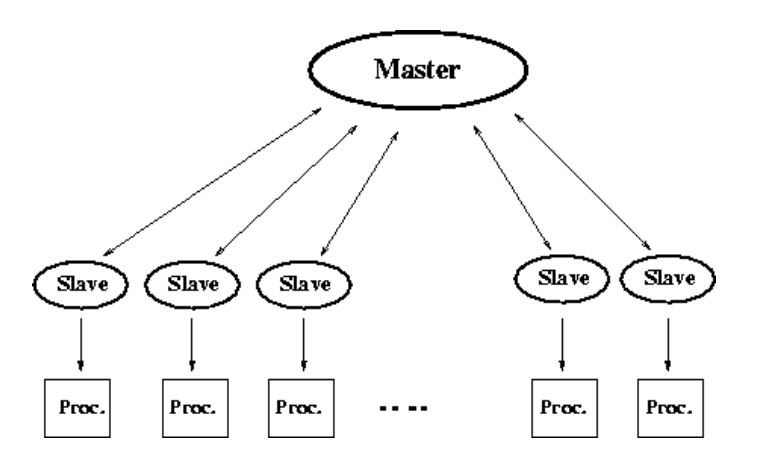
\includegraphics[width=0.5\textwidth]{Figure1.png}}
    \caption{Diagram of basic Master Slave Data Flow \cite{ramaekers}}
    \label{Figure1}
\end{figure}

A master-slave relationship is a network where one computer acts as a master, and gives instructions to many slave computers which will report back to their master, see \ref{Figure1}. This setup can be extremely useful for performing computationally intensive tasks as mentioned above. This is because if the task can be broken up into multiple smaller tasks, then they can be ran concurrently using the computational resources in the network. Sockets are used to transmit data between each node in the network. The downside to this approach is that it can often require much more overhead to run efficiently. The master node in the network must be able to efficiently send instructions to its slave nodes and be able to patch together each result of the smaller tasks into a single result that solves the large problem, and this can be difficult to implement.

\subsection{Peer to Peer Relationships}
Peer to peer (P2P) networks operate in a different structure than master-slave networks. A P2P network is completely decentralized, and all nodes in the network operate as equals \cite{milojicic2002peer}. One notable example of a P2P network is torrenting. In a torrent network, there can be many thousands of nodes in the network that both share files, and request files from other nodes. This setup has advantages over a master-slave network. One notable advantage is that there can often be more reliability with these networks. There is no single point of failure as the system as a whole can function even if one node goes down. Another advantage can be seen in the cost to setup these systems. Since the goal of P2P networks is often to decentralize a network, one can lower the cost of ownership for being part of the network since no one person needs to be in control of the network \cite{milojicic2002peer}.
\begin{figure}[H]
    \centering
    \centerline{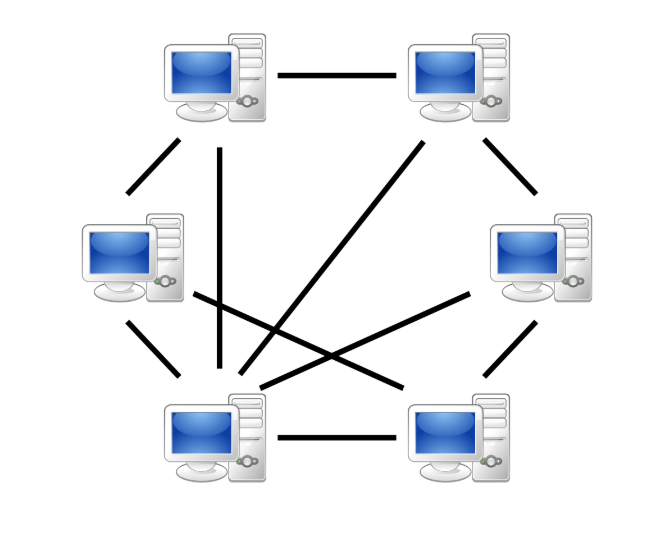
\includegraphics[width=0.5\textwidth]{Figure2.png}}
    \caption{Diagram of P2P network \cite{bieg_2007}}
    \label{Figure2}
\end{figure}

\section{Security}
As with most aspects of the internet today, security is an issue that cannot be ignored when discussing web sockets. Even though the standard has been around for decades, it has not been reliably or adequately updated to protect against modern security threats. This is due to many complicating factors that are outside the scope of this paper. However, below are some examples of both commonly exploited and uncommonly exploited vulnerabilities in the socket communication protocol as well as potential experimental solutions.

\subsection{Vulnerabilities}
\subsubsection{No Built-In Security Measures}
There is no security built into the socket protocol. This means that all applications that use sockets must be designed to protect against any and all possible attack vectors. Some protections are given by host operating systems; however, they are not all-inclusive and not always sufficient. This results in inconsistent security practices among applications who utilize sockets and an inability to quickly fix a security problem as many organizations must act separately to solve any security concerns.

At the Black Hat conference of 2009 a security researcher gave a presentation where they showed how simple it was to intercept Secure Socket Layer (SSL) traffic and compromise a user’s secret login data by performing a man-in-the-middle style attack \cite{sheble_2009}. This traffic would be traveling across a socket from the user’s machine to the login server. Due to the fact that information traveling over sockets is not encrypted or otherwise protected by default. This researcher was able capture essentially all data that users were entering to the compromised website.

The attack was only able to be carried out when users were moving from an unsecured http page to a secured https page to log into the compromised service. The researcher was then able to intercept and reroute traffic to their proxy server before directing the traffic to its original destination \cite{sheble_2009}. If the socket protocol included ways to verify that traffic had not been intercepted on its way to a destination or encrypted all information sent over a socket by default, this attack would not be able to be carried out.


\subsubsection{Blind Trust}
Due to the fact that operating systems protect I/O devices from being directly accessed by applications, the applications must trust that the host operating system is delivering data exactly as it appeared over the socket \cite{ta2006splitting}. This is typically not an issue, however in cases where the host operating system has been taken over by a malicious entity or otherwise compromised, problems quickly arise.

Traditional computers and operating systems have no workable solution to this problem. Therefore, a new type of computer operating system called Proxos was developed by researchers at the University of Toronto with the specific goal of addressing this blind trust problem.

\begin{figure}[htbp]
    \centering
    \centerline{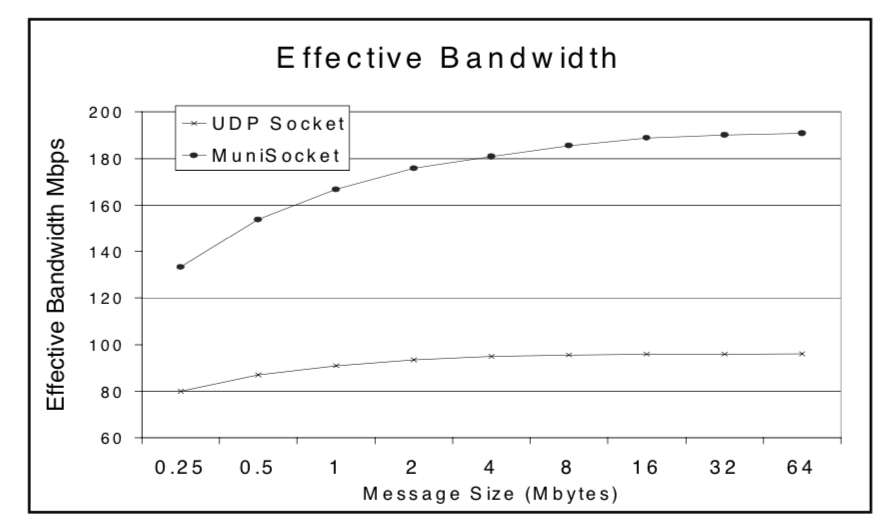
\includegraphics[width=0.5\textwidth]{Figure3.png}}
    \caption{Diagram of the Proxos System Architecture \cite{ta2006splitting}}
    \label{Figure3}
\end{figure}

As can be seen in the above figure, this system architecture is made up of three or more Virtual Machines (VM). The Virtual Machine Master (VMM) would be responsible for overseeing all other virtual machines that operate on the system. It would also be responsible for allocating resources to each VM as they are created or destroyed \cite{ta2006splitting}. It is not a traditional operating system. It is only intended to manage hardware resources and respond to requests made to those resources. The Commodity Operating System (OS), the researchers used Linux, would be what we are used to today, the traditional user operating system. It would be allowed to run application as any other normal operating system would. The only difference is that it is not responsible for handling hardware resources and can only ask the VMM for the resources it needs \cite{ta2006splitting}.

The main difference between Proxos and traditional computer systems lies in how it handles applications that want to have more security. These applications are given their own private VM with their own copy of the OS that can make trusted calls directly to the VMM and bypass a potentially compromised host operating system. Only the application is allowed in this private VM. Its application-trusted system calls are allowed to communicate directly with the VMM to get information directly from hardware resources while untrusted system calls are sent back to the Commodity OS\cite{ta2006splitting}. This means that, regardless of if the host operating system that the user is running can be trusted, programs running in this private VM environment can be sure that there are no security risks in their application or operating system scope as there is no way for the VMM to be compromised.

According to the paper published by the researchers this enormous gain in security came with only minimal performance reduction when compared to running identical applications on Linux. Furthermore, existing applications were able to be modified to work with this system with modifying very little code (as few as 10s of lines).

\subsubsection{Distributed Denial of Service Attacks}
Distributed Denial of Service (DDoS) attacks are simple in purpose and in execution. They are designed to disrupt communication over a network. They do so by using multiple hosts to disrupt communication by overloading a socket with bogus information requests or other meaningless traffic \cite{herbert2015ddos}.

Unfortunately, sockets are designed to take and process all information that is assigned They, and therefore the targeted system alone, are defenseless against this style of attack. To further complicate the detection and prevention of DDoS attacks, the attacking host(s) may inaccurately report (spoof) the socket that the traffic originates from, therefore the targeted system is unable to determine which requests are legitimate and which requests are from an attacking system \cite{herbert2015ddos}.

\subsection{Potential Solutions}
Many companies and researchers have come up with solutions to address the security vulnerabilities of sockets. Some of these solutions have been widely adopted, such as rate limiting, while others, such as artificial intelligence (AI) or neural network based approaches, are beginning to be adopted by the industry and end users. What follows is a summary of some ways the many security vulnerabilities of sockets can be addressed.

\subsubsection{Traffic Filtering}
Many network routing and switching appliances come with software solutions to protect against common socket exploits. Most commonly, these network appliances limit the number of requests that that can be made from or to clients in order to ensure fair network use amongst all clients \cite{herbert2015ddos}. While the real intent is to provide fair network access, some protection is given to against DDoS attacks as a side effect. This is due to the fact that sockets are less likely to be overwhelmed by excessive traffic as the flow rate of traffic is modified as the rate of requests from one or to one source is limited.

\subsubsection{Smart Wire}
This is a concept where a monitoring device is inserted on a normal communication wire and passively monitors the traffic that passes across the wire \cite{herbert2015ddos}. When the monitoring device detects a threat of any sort, it can update routers, firewalls, and even antivirus software that a threat is being transferred and pinpoint its source and destination sockets. This would allow systems on the network to be warned about the attack and take any appropriate defensive measures (such as blocking traffic from the originating socket).

This technique only works when the monitoring device is able to monitor traffic without creating a bottleneck and thereby reducing the throughput of the smartwire. Additionally, precautions must be taken to ensure that the monitoring device is not compromised. Because it sits between source and destination sockets, it is in the perfect place to execute a man-in-the-middle attack such as redirecting traffic to another destination or stealing private information that may be transferred across the smart wire.

\subsubsection{Agent Based Threat Detection}
Another common way to detect threats is to use agents. In this setup each network device would have a copy of the base model used to determine if traffic (or any other activity) is a threat. The threat detection artificially intelligent agents would periodically scan to determine if any suspicious activity is occurring and respond as necessary.

There are many benefits to using agents as threat detection tools. One is that there may be multiple agents working to accomplish the same task or each may be specialized to perform a subset of the larger task \cite{arabo2019distributed}. One example of this could be one agent being used to detect active network threats coming across a socket such as DDoS attacks while another is looking for more passive threats such as port scans. This allows information to be processed more quickly and at a more granular level as opposed to a non-agent based approach \cite{arabo2019distributed}. Another benefit is the ability for a network of many deployed agents to learn independently as they differing types of attacks and update each other with the knowledge they gain detecting attacks. This is the approach that is taken by many modern-day antivirus applications \cite{arabo2019distributed}.

\section{Experimental Uses}
There are many ways that researchers are attempting to adapt or improve the traditional idea of a socket. Because the socket is so widely used and is not owned by any particular organization or individual adaptations and improvements are essentially risk free and have the potential to impact a wide variety of users. What follows is a summary of one innovative idea and how it may impact the future of network based communication.

\subsection{MuniSocket}
This is an experimental middle-layer API that can allow one socket to be used on multiple network interfaces \cite{mohamed2002user}. The problem that it can solve is the need for large data transfers to be done more rapidly. As of now, most network transfers come from one source socket and go to one source socket. Due to the limitation that a socket can only be active on one network device at a time, this significantly limits the speed at which data can be transferred.


\begin{figure}[htbp]
    \centering
    \centerline{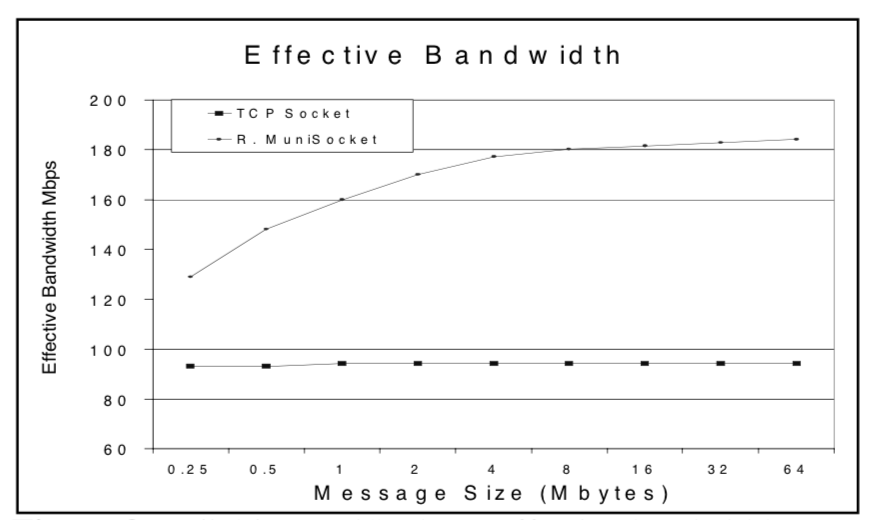
\includegraphics[width=0.5\textwidth]{Figure4.png}}
    \caption{Diagram of the UDP version of a MuniSocket \cite{mohamed2002user}}
    \label{Figure4}
\end{figure}

As you can see in Figure \ref{Figure4} the MuniSocket allows for applications to act as if they are interfacing with one socket directly and then subdivides all traffic to be transferred over a socket to one or more network interfaces. This results in three main benefits. The speed of the transfer is increased due to more throughput potential, it becomes possible to balance the load of network cards, and fault tolerance becomes more feasible as the MuniSocket is able to re-route the traffic without the application knowing that a fault has occurred \cite{mohamed2002user}.

The MuniSocket can operate in both a UDP and TCP configuration \cite{mohamed2002user}. This is due to the fact that the MuniSocket still uses the traditional socket protocols to transfer data. Both the reliable TCP and unreliable UDP MuniSockets saw similar performance in terms of data transfer speed to their traditional counterparts. Both the TCP and UDP configurations of the MuniSocket were found to have a higher throughput capacity than their respective traditional counterpart (see \ref{Figure5} and \ref{Figure6}) \cite{mohamed2002user}. The paper offered no explanation as to why this may be but it is reasonable to assume that this is due to the increased throughput capacity of having multiple network interfaces.

\begin{figure}[htbp]
    \centering
    \centerline{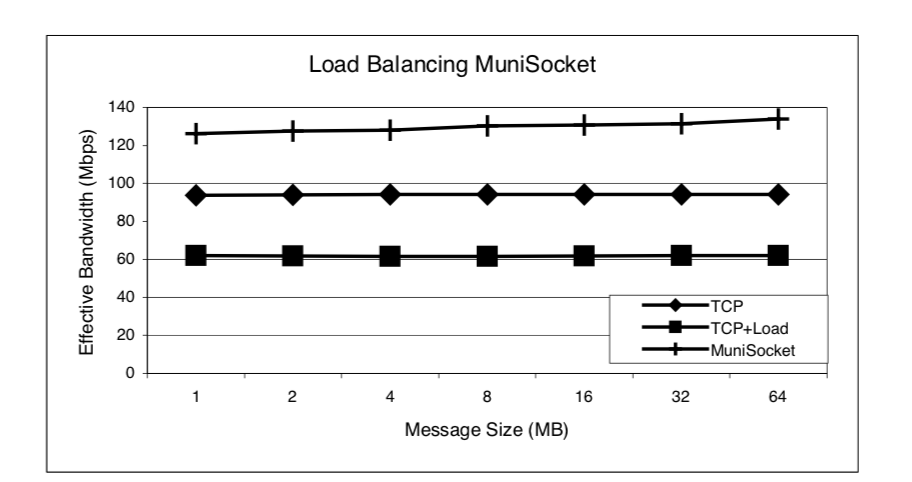
\includegraphics[width=0.5\textwidth]{Figure5.png}}
    \caption{Results of testing UDP MuniSocket bandwidth \cite{mohamed2002user}}
    \label{Figure5}
\end{figure}
\begin{figure}[htbp]
    \centering
    \centerline{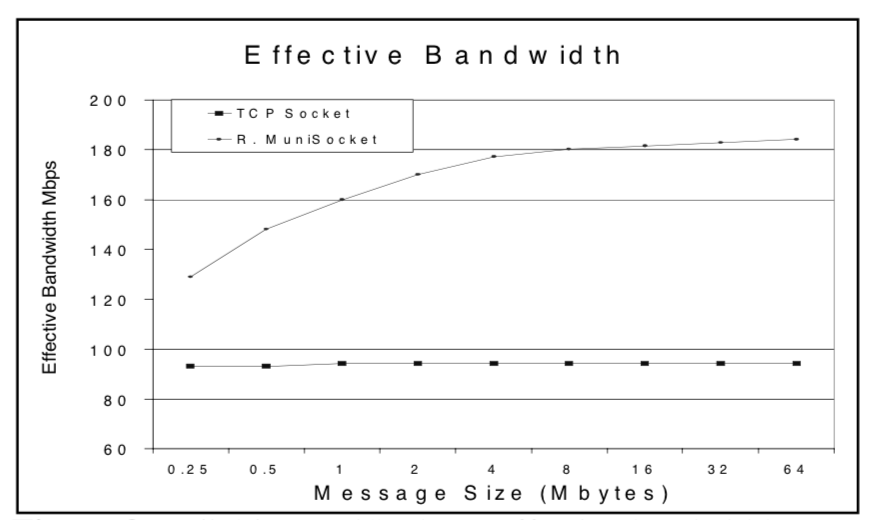
\includegraphics[width=0.5\textwidth]{Figure6.png}}
    \caption{Results of testing TCP MuniSocket bandwidth \cite{mohamed2002user}}
    \label{Figure6}
\end{figure}

Although this technology seems promising and is an innovative way to interface with sockets testing revealed that only moderate performance gains were possible with the current implementation. Figure \ref{Figure7} shows that in the tests performed only slight increases in transfer speeds were observed when using multiple interfaces to balance the load of the transfer. It is possible that this was due to the artificial nature of the test and real-world scenarios would reveal better results. Nevertheless, the minimal performance gains do not inspire hope that the MuniSocket will be widely adopted.

\begin{figure}[htbp]
    \centering
    \centerline{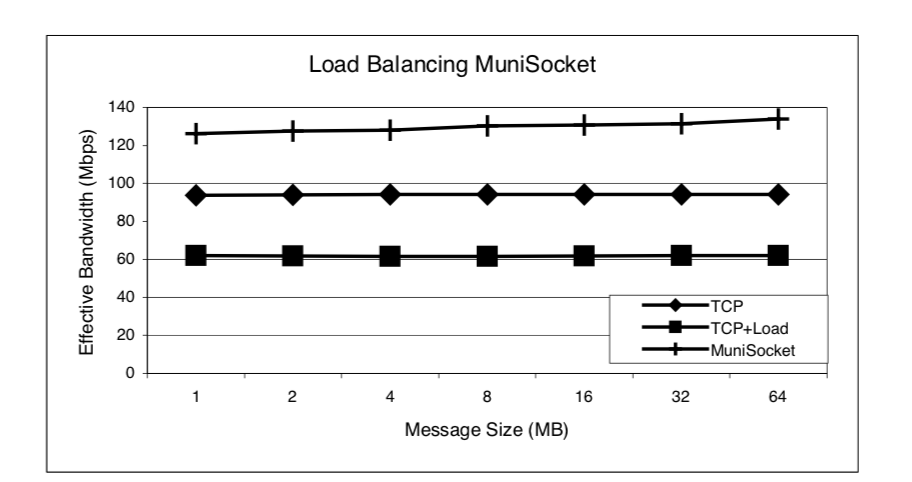
\includegraphics[width=0.5\textwidth]{Figure7.png}}
    \caption{Results of load balancing test for MuniSocket \cite{mohamed2002user}}
    \label{Figure7}
\end{figure}

\section{Comparison}
\subsection{Pipes}
Pipes, a befitting name to serve their purpose, are used to connect the output of a process to the input of another process, and sockets are used to send data between different IPv4/IPv6 endpoints. Pipes only exist within a specific host whereas sockets can extend beyond localhost depending upon the need (could be local for interprocess communication but needs to be beyond that for distributed computing). Pipes and sockets both transfer data as byte streams.

\subsection{Remote Procedure Calls}
Remote Procedure Call (RPC) is a protocol that can be used to request a service from a program located in another node on a network without having to understand the network’s details. It is also called a function call or a subroutine call \cite{techtarget_2016}. It uses the client-server model and is a synchronous operation requiring the requesting program to be suspended until the results of the remote procedure are returned. Sockets are a way of implementing remote procedure call services, and are quite low level compared to RPCs, which hide the communication details behind procedural calls. The use of RPC compilers allows for the communication protocol to be generated automatically from the interface description.

\begin{figure}[H]
    \centering
    \centerline{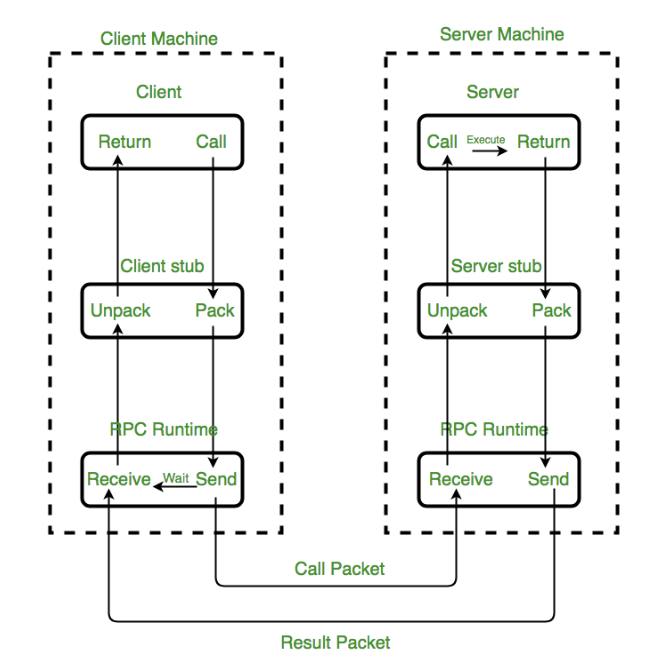
\includegraphics[width=0.5\textwidth]{Figure8.png}}
    \caption{Results of load balancing test for MuniSocket \cite{geeks}}
    \label{Figure8}
\end{figure}

\section{Conclusion}
Clearly sockets are deeply embedded into computer systems around the globe. Without them, modern life would look very different. Perhaps because of their widespread use and because of their potential to be a single point of failure for internet communication they have been targeted by many different styles of attacks. This makes sockets both essential and a thorn in the side of programmers everywhere. As was illustrated in this paper, there are both simple and innovative solutions to repair the shortcomings of sockets. Proxos seems to be the most promising due to its reliance on the traditional socket implementation and innovative sectioning approach to information flow. All other solutions seem to have the downfall of not being backward compatible with the existing socket implementation. While it is a monumental task, it seems as though it is time to address the aging socket standard. With security and privacy being a major concern in today’s climate, the socket is an attack vector that is too easy to exploit. New security features such as encryption, user verification, and measures to ensure message integrity are essential. Without them, we will be forced to continue trying to stop exploits without addressing the main problem.

\bibliography{workscited.bib}
\bibliographystyle{ieeetr}

\end{document}
